\documentclass[]{article}
\usepackage[nodayofweek,level]{datetime}
\usepackage{hyperref}
\usepackage{listings}
\usepackage{centernot}
\usepackage{amsmath,amssymb}
\usepackage{graphicx}
\newcommand{\rithm}{\textbf{RiTHM}\space}

% Title Page
\title{\rithm development status report}
\author{}


\begin{document}
\maketitle

\begin{abstract}
Details about the current progress of \rithm development and journal paper
\end{abstract}
\section{Current Results and Details about on-going items}


	\subsection{Runtime verification in case of Missing Events}
	\begin{itemize}
	
	\item \textbf{Missing Events} correspond to the case when Runtime Monitor does not receive a trace from the program which is being monitored.
	
	\item Events could be missed for a \emph{finite} amount of time or there could be \emph{persistent}. This loss of a stream of events could be formalized as either a \emph{finite} path within the program when the events could not be monitored or a possible \emph{infinite} path within the program when the events could not be monitored.
	
	\item In case of loss of trace for \emph{finite} time, the monitor cannot keep track of a finite path which is being executed in the program and hence it cannot provide verdict of certain type of \emph{LTL} properties.
	
	\item On the other hand, a \emph{persistent} loss of program trace implies that the monitor cannot validate any type of \emph{LTL} property.
	
    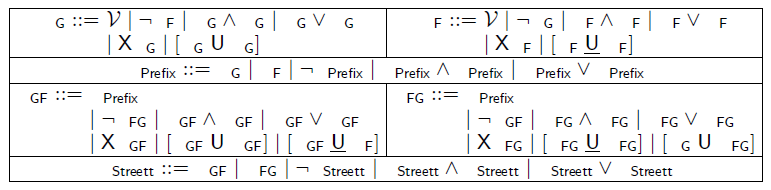
\includegraphics[scale=0.4]{LTLHierarchy.png}
    
    \item In above, \emph{LTL} hierarchy, there are 6 classes of specifications and the class \emph{Street} is the most expressive one and for most of the LTL formulae, it is not difficult to find an equivalent class which belongs to the class \emph{Street}.
    
    	\item Among the classes in \emph{LTL} hierarchy, in the event of loss of trace for a \emph{finite} path within the program, it is not possible to preserve soundness while monitoring \emph{Safety $(P_G)$}, \emph{Liveness $(P_F)$} and \emph{Prefix} which is boolean closure of \emph{Safety} and \emph{Liveness}
    
    \item This happens because a \emph{Liveness} property could be satisfied by a \emph{finite} path of a \emph{reactive} system and a \emph{Safety} property could be violated by \emph{finite} path. This \emph{finite} path could be the path whose trace was lost. Hence, the verdict given by a \emph{LTL} monitor might not show the actual status.
    
    \item On the other hand, the properties in the class \emph{Recurrence ($P_{GF}$)} and \emph{Persistence ($P_{FG}$)} could be monitored by tolerating a loss of trace for a \emph{finite} path in the program provided certain criteria are fulfilled by states of \emph{LTL} monitor.
    
    \item The formulas which belong to the class \emph{Recurrence ($P_{GF}$)} have B\"{u}chi acceptance condition where one of the final states if the B\"{u}chi automaton should visited by the run of infinite word infinitely often. Hence, a \emph{finite} loss of program trace would not affect the monitoring provided the monitor (which is constructed from B\"{u}chi automaton) visits one of the final states infinitely often.
    
    \item The formulas which belong to the class \emph{Persistence ($P_{FG}$)} have Persistence acceptance condition where one of the final states if the Persistence automaton should be continuously visited by the run of infinite word. Hence, a \emph{finite} loss of program trace would not affect the monitoring provided the monitor eventually visits one of the final states in a continuous manner.
    
    \item \emph{Strett} class, which is boolean closure of \emph{Persistence} and \emph{Recurrence} classes exhibits a combination of acceptance conditions of \emph{Persistence} and \emph{Recurrence}. 	
    
    \item For example., below LTL$_4$ monitor belongs to the \emph{Persistence} property $\diamondsuit \square a$ U $b$. Here, provided the monitor is in one of the states among (0,1), (1,0), (1,1), a finite loss of a stream of events could be tolerated without violating the \emph{asymptotic} evaluation the truth value of the formula. 
     
    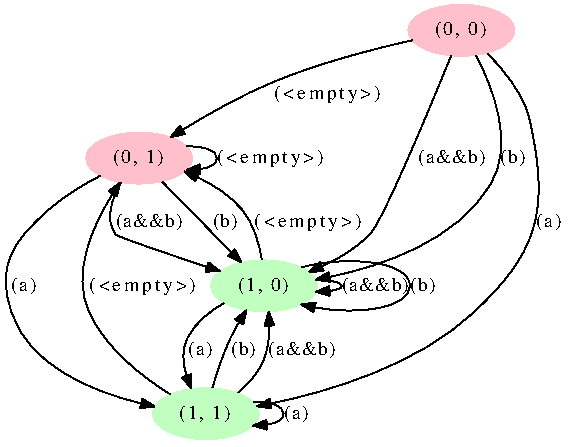
\includegraphics[scale=0.6]{FGExample.png}
    
    \item Below LTL$_4$ monitor belongs to the \emph{Recurrence} property $\square \diamondsuit  a$ U $b$. Here, provided the monitor is in one of the states among (0,1), (1,0), a finite loss of a stream of events could be tolerated without violating the \emph{asymptotic} evaluation the truth value of the formula. 
    
    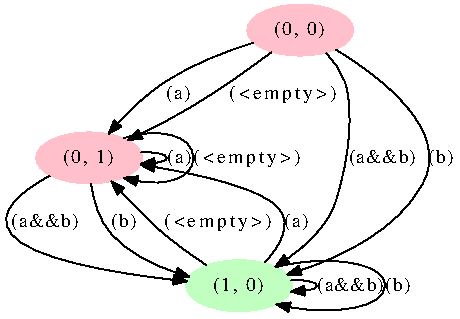
\includegraphics[scale=0.6]{GFExample.png}
    
    \item Future directions can include the proof of asymptotic correctness of the valuation of truth-value in the event of \emph{finite} loss of trace for  \emph{Recurrence ($P_{GF}$)}, \emph{Persistence ($P_{FG}$)} and \emph{Strett} classes.
    
    \end{itemize}
	\subsection{\rithm development work}
	\begin{itemize}
	\item MTL parser has been developed, the monitor for MTL is being developed. \textbf{Update}: Including both Past-time and future-time MTL variants. 
	\item For developing predicate specification language, work is done on analysis of script engines which can be used. Beanshell \url{http://www.beanshell.org/intro.html} is under consideration along with JavaScript engines which can be embedded into java code, and the predicate definitions could be specified using the languages of these engines.
	
	\item IronForge data, and running \rithm on the properties of the data. Work in Progress.
	
	\item Integration of DIME + \rithm - Papers worked on for analyzing the previous work. Work done by Smolka et al. focuses on using Markov Chains for providing probabilistic estimates on the satisfaction of specifications. On similar lines, Probabilistic Timed Automata could be used for specifying 
	models of systems which exhibit the characteristics of incomplete-data for verification along with the requirement of hard real-time deadlines.
	\item 'Lessons Learnt' section for journal paper is being worked upon.
	
	\item \rithm's monitor using specifications in the format of regular expressions is being enhanced so that monitoring is trace-length independent. The coding is in progress and we now use \url{http://www.brics.dk/automaton/doc/index.html} to create automaton from regular expression and input trace ti this automaton event by event. 
	

	

	\end{itemize}
	
\section{Previous Results}
\begin{itemize}
\item 
	\rithm For CRV'15 competition which will be held with RV'15 conference, benchmarks are submitted for 'C' program monitoring track and Offline Monitoring track.
	The details of benchmarks which are submitted can be found at 
	\begin{itemize}
		\item For 'C' program monitoring track - \url{https://forge.imag.fr/plugins/mediawiki/wiki/crv15/index.php/C_track}
		\item For Offline monitoring track \url{https://forge.imag.fr/plugins/mediawiki/wiki/crv15/index.php/Offline_track}
	\end{itemize}
	\item The 'C' program benchmarks are designed to monitor a 'C' program which launches 0.1 million POSIX threads, and various properties have been specified using First Order Linear Temporal Logic (Past as well as Future time)
	\item 'C' program which is being monitored can be found at \url{https://github.com/yogirjoshi/CRVBenchMark}
	\item The specifications for 'C' program monitoring track are as per below
	\begin{itemize}
		\item $\forall$ tid: pthread\_create(tid) $\longrightarrow$ $\diamondsuit$ pthread\_running(tid)
		\item $\forall$ tid: pthread\_mutex\_lock(tid, "ex\_mutex") $\longrightarrow$ $\diamondsuit$ pthread\_mutex\_unlock(tid, "ex\_mutex")
		\item $\forall$ tid: pthread\_create(tid) $\longrightarrow$ $\diamondsuit$ pthread\_join(tid)
		\item $\forall$ tid: (pthread\_mutex\_lock(tid, 'ex\_mutex') $\vee$ pthread\_mutex\_destroy(tid, 'ex\_mutex') $\vee$ pthread\_mutex\_unlock(tid, 'ex\_mutex')) $\longrightarrow$ $\diamondsuit^{-1}$ pthread\_mutex\_init(10000, 'ex\_mutex')))
		\item $\forall$ tid: (pthread\_exit(tid)) $\longrightarrow$ $\diamondsuit^{-1}$ pthread\_mutex\_unlock(tid, 'ex\_mutex'))
	\end{itemize}
	\item For offline monitoring track, QNX trace-logger files have been used. The trace file is at \url{https://github.com/yogirjoshi/datatools/blob/master/CRV1.tar.gz}. It contains 0.1 million events on which the specifications will be validated.
	\item Specifications are defined on various events of QNX threads. The specifications are as per below
	\begin{itemize}
		\item $\forall$  pid, $\forall$ tid : (thcreate $\longrightarrow$  $\diamondsuit$ thrunning)  (Satisfied by trace)
		\item $\forall$ $>90\%$ pid, $\forall$ tid : ($\diamondsuit$ threply) - Vioated by trace
		\item $\forall$  pid, $\forall$ tid : ($\square$ (thready $\longrightarrow$   $\diamondsuit$ thrunning)) - Satisfied by trace
		\item $\exists$ $=1$ pid, $\exists$ $=2$ tid: $\lnot$ ($\square$ ( $\lnot$ thdestroy)) - Vioated by trace
		\item $\forall$ $>50\%$ pid, $\forall$ $>50\%$ tid: ( $\diamondsuit$ ( thsem $\vee$ thmutex ) ) - Vioated by trace
	\end{itemize}
	
\item
Verbose LTL parser is implemented which uses verbose representation of LTL operators. \newline
The code is at \url{https://github.com/yogirjoshi/parsertools.git}.

\item
Verbose LTL parser is integrated with existing LTL monitor. Some new APIs added to Parser interface for rewriting the specifications into interchangable formats. The code is at \url{https://github.com/yogirjoshi/monitortools.git}

\item
\rithm plugin loader is implemented so that different monitors, parsers and data-importers can be plugged in and used. \newline
Below example starts \rithm instance to monitor LTL specifications using four valued semantics, and it uses CSV data
\begin{lstlisting}
java rithm.driver.RiTHMBrewer 
-specFile=/home/y2joshi/InputFiles/specsQnx 
-dataFile=/home/y2joshi/Input1.csv
-outputFile=/home/y2joshi/InputFiles/output3.html 
-monitorClass=LTL4 
-traceParserClass=CSV 
-specParserClass=LTL
\end{lstlisting}
Similarly, \rithm's another instance can be started to monitor using Verbose LTL (using 4-valued semantics), and it uses trace data in XML format 
\begin{lstlisting}
java rithm.driver.RiTHMBrewer 
-specFile=/home/y2joshi/InputFiles/specsQnx 
-dataFile=/home/y2joshi/Input1.XML
-outputFile=/home/y2joshi/InputFiles/output3.html 
-monitorClass=LTL4 
-traceParserClass=CSV 
-specParserClass=VLTL
\end{lstlisting}


\item \rithm can import data in CSV format and the CSV data-importer is intergrated with \rithm framework

\item
\rithm source has been refactored to use maven for project source code and build management. \rithm source has been enhanced to drop some legacy APIs to make the design more scalable

\item API key feature for \rithm is being implemented. The API key will allow access management for \rithm when used in server mode.
\end{itemize}
\end{document}      
